\documentclass{article}
\usepackage{ctex} % For Chinese characters
\usepackage{amsmath} % For mathematical environments and symbols
\usepackage{graphicx} % For including images (placeholders here)
\usepackage{geometry} % To adjust page margins
\usepackage{hyperref} % For clickable links in the table of contents
\usepackage{booktabs} % For professional looking tables (optional, but good practice)
\usepackage{float} % For the [H] float placement specifier
\usepackage{caption} % For better caption handling
\usepackage{biblatex} % For bibliography management
\geometry{a4paper, margin=1in} % Adjust margins as needed

\title{激光拉曼光谱}
\author{
    郑晓旸 20211030007\\
    指导老师:  何聪丽
}
\date{2025年5月21日}

\begin{document}

\maketitle

\tableofcontents

\newpage % Start content on a new page

\section{实验}

本实验采用半导体激光器泵浦的 Nd$^{3+}$:YVO$_{4}$ 晶体并倍频后到的 532nm 激光作为激发光源, 研究液体样品 CCl$_{4}$ 分子的拉曼光谱。

\subsection{光子计数器阈值设定}

启动计算机后, 先打开激光光谱仪的开关, 再运行拉曼光谱仪的测量程序, 等待光栅初始化完成后, 在阈值窗口测量无光时的暗计数与脉冲幅度的分布曲线。选择合适的阈值, 将其输入到主程序左侧界面的阈值窗口。

\subsection{初步测量拉曼光谱}

\subsubsection{参数设置}

工作方式: 波长; 间隔: 0.1nm; 工作范围: 起始波长: 510nm, 终止波长: 560nm; 最大值: 100000, 最小值: 0; 负高压: 8; 域值: 14; 积分时间: 800ms。确认光栅狭缝处于合适宽度。

\subsubsection{粗扫}

粗调光路之后, 令单色仪从 510nm 开始单程扫描, 得到初步测量的拉曼光谱。

\subsection{细调光路}

在峰位处定点扫描, 同时调整光路, 使得接收到的散射光强增大, 在电脑图像上表现为光强曲线随时间上升。

再在 532nm 的瑞利散射峰附近和 555nm 的双峰附近反复扫描, 改变狭缝的大小, 直至瑞利散射峰顶端尖锐、双峰尽量高且能分开。

\subsection{精细测量拉曼光谱}

光路优化完成后, 再次从 510nm 至 560nm 扫描, 即可得到精细测量的拉曼光谱。利用自动寻峰功能, 可以快速峰值和峰位信息。

\subsection{退偏度的计算}

为了定量描述散射光相对入射光偏振态的改变, 我们引入退偏度的概念。定义入射光的传播方向和散射光的观测方向构成的平面为散射平面, 引入符号 $I_\perp(\theta)$ 描述散射光强度, i 和 s 分别表示入射光和散射光的偏振方向相对于散射平面的取向。垂直于散射平面标记为 $\perp$, 平行于散射平面标记为 $\parallel$, 自然光标记为 n。退偏度定义为偏振方向垂直和平行于入射光偏振方向的散射光强之比。

在光路中加上偏振片, 旋转检偏器, 扫描检偏器相互垂直时的两种拉曼散射谱线。计算退偏度, 并记录在表 2 中。

\subsection{单光子计数器的进一步研究}

点击“检索”, 使单色仪光栅处于拉曼光谱的某一峰值附近。在激光开启的情况下, 再次打开阈值窗口, 测量此时的脉冲计数与脉冲幅度的分布曲线, 并与之前的结果作比较。

\section{结果与分析讨论}

\subsection{阈值设定}

无光时暗计数与脉冲幅度分布曲线如图 1 所示, 此时激光并未开启, 图像中的峰源自光电倍增管的热噪声。选取阈值为 14 以滤去后续测量中热噪声的影响。

\begin{figure}[H]
    \centering
    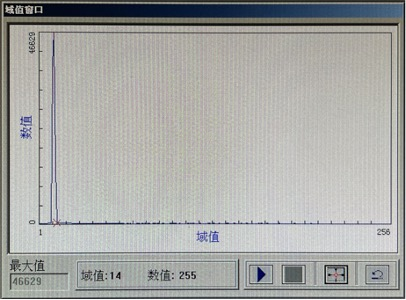
\includegraphics[width=0.8\textwidth]{图片 1.jpg} % Placeholder for Figure 1
    %\rule{0.8\textwidth}{3cm} % Placeholder box
    \caption{无光时 PMT 输出的脉冲分布曲线}
    \label{fig:pmt_dark_count}
\end{figure}

\subsection{拉曼光谱的初步测量}

\subsubsection{粗调光路}
1. 先不加偏振片, 打开激光电源, 细调样品架和样品池的位置, 使激光束处于柱形样品池的轴线上。从各水平方向观察, 确认样品处在最佳照射状态。
2. 反复调节成像透镜组的前后位置, 使激光束腰在单色仪狭缝处成像最细最清晰。
3. 调节凹面镜的前后左右和俯仰角, 使被反射的散射光沿激光束腰和在狭缝上的像的中心连线汇聚到样品池中心, 以增加进入单色仪的拉曼散射光强。

\subsubsection{光谱粗扫}

参数设定完成后, 在 510nm-560nm 范围内进行扫描, 得到拉曼光谱的初步测量图像, 如图 2 所示。可以看到此时中心的瑞利散射峰非常宽, 说明光路和狭缝还需要进一步调整。

\begin{figure}[h]
    \centering
    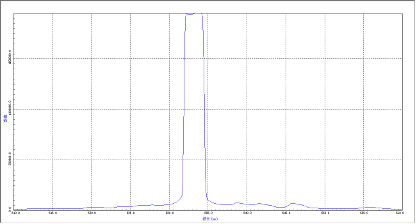
\includegraphics[width=0.8\textwidth]{图片 2.png} % Placeholder for Figure 2
    % \rule{0.8\textwidth}{3cm} % Placeholder box
    \caption{拉曼光谱的初步测量结果}
    \label{fig:rough_scan}
\end{figure}

\subsection{光路的优化}

利用“定点”功能测量固定波长的光强随时间的变化, 并在此期间微调光路, 使接收到的散射光增多, 光强变化趋势见图 3。

\begin{figure}[h]
    \centering
    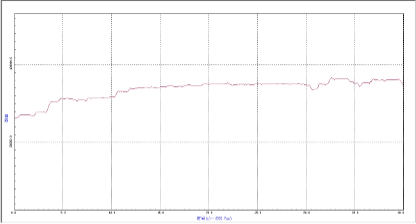
\includegraphics[width=0.8\textwidth]{图片 3.png} % Placeholder for Figure 3
    % \rule{0.8\textwidth}{3cm} % Placeholder box
    \caption{优化光路使接受到的散射光不断增强}
    \label{fig:optimization}
\end{figure}

接着在 532nm 的中心瑞利散射峰和 555nm 的双峰附近小范围扫描, 调节狭缝的宽度, 使瑞利散射峰顶端尖锐、双峰尽量高且能分开。细锐的瑞利峰和分开的双峰如图 4 和 5 所示, 此时确定合适的狭缝大小为 0.2mm。

\begin{figure}[h]
    \centering
    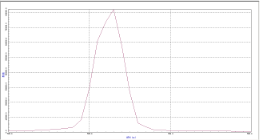
\includegraphics[width=0.45\textwidth]{图片 4.png} % Placeholder for Figure 4
    % \rule{0.45\textwidth}{3cm} % Placeholder box
    \quad
    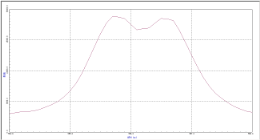
\includegraphics[width=0.45\textwidth]{图片 5.png} % Placeholder for Figure 5
    % \rule{0.45\textwidth}{3cm} % Placeholder box
    \caption{图4: 细锐的瑞利散射峰 \quad 图5: 555nm 附近分开的双峰}
    \label{fig:narrow_peaks}
\end{figure}


\subsection{拉曼光谱的精细测量}

光路优化完成后, 再次从 510nm-560nm 扫描, 得到精细测量的拉曼光谱, 见下图 6。对比图 6 和之前粗扫得到的图 2, 可以看到中心的瑞利散射峰明显变细, 两侧的拉曼散射峰也更为明显。图 7 是图 6 的局部放大并自动寻峰后的结果, 从中可以更清晰地看到拉曼散射峰。图中明显的峰共有 9 个, 位于中心的瑞利散射线在强度上远高于周围的拉曼散射线。拉曼线的峰位在瑞利线两侧呈对称分布, 强度极弱, 低频一侧 (右侧) 的谱线为 Stokes 线, 高频一侧 (左侧) 的为反 Stokes 线。在 556nm 附近可观察到分开的双峰。峰位和峰高记录在表 1 中。

\begin{figure}[h]
    \centering
    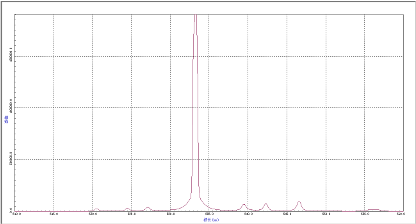
\includegraphics[width=0.8\textwidth]{图片 6.png} % Placeholder for Figure 6
    % \rule{0.8\textwidth}{5cm} % Placeholder box
    \caption{拉曼光谱的精细测量}
    \label{fig:fine_scan}
\end{figure}

\begin{figure}[H]
    \centering
    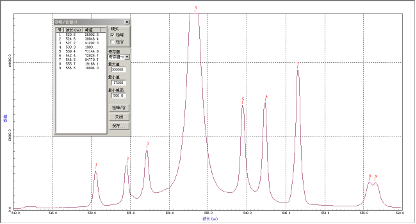
\includegraphics[width=0.8\textwidth]{图片 7.png} % Placeholder for Figure 7
    % \rule{0.8\textwidth}{5cm} % Placeholder box
    \caption{拉曼光谱的精细测量(放大并寻峰)}
    \label{fig:fine_scan_zoom}
\end{figure}


\begin{table}[h]
    \centering
    \caption{峰值和峰位}
    \begin{tabular}{cccccccccc}
        \toprule
        峰编号 & 1 & 2 & 3 & 4 & 5 & 6 & 7 & 8 & 9 \\
        \midrule
        峰位 (nm) & 520.5 & 524.6 & 527.2 & 533.3 & 539.4 & 542.4 & 546.5 & 555.7 & 556.5 \\
        \hline
        峰值 & 26902.8 & 30846.4 & 41292.3 & - & 71144.9 & 72825.7 & 94770.7 & 19166.1 & 18894.0 \\
        \bottomrule
    \end{tabular}
    \label{tab:peak_values1}
\end{table}


\subsection{退偏度的测量}

实验中的光路图如下图 8 所示, 其中红色双向箭头代表光的偏振方向。旋转检偏器测量光强, 发现检偏器的透光方向为 90$^\circ$/270$^\circ$ 方向。检偏器置于 0$^\circ$/180$^\circ$ 时, 测得的光谱是图 9 中的蓝线; 检偏器置于 90$^\circ$/270$^\circ$ 时, 测得的光谱是图 9 中的红线。图 10 是图 9 的局部放大, 从中可以更清晰地看到拉曼光谱的变化。利用寻峰工具, 记录下各个峰高, 整合在表 2 中。

\begin{figure}[h]
    \centering
    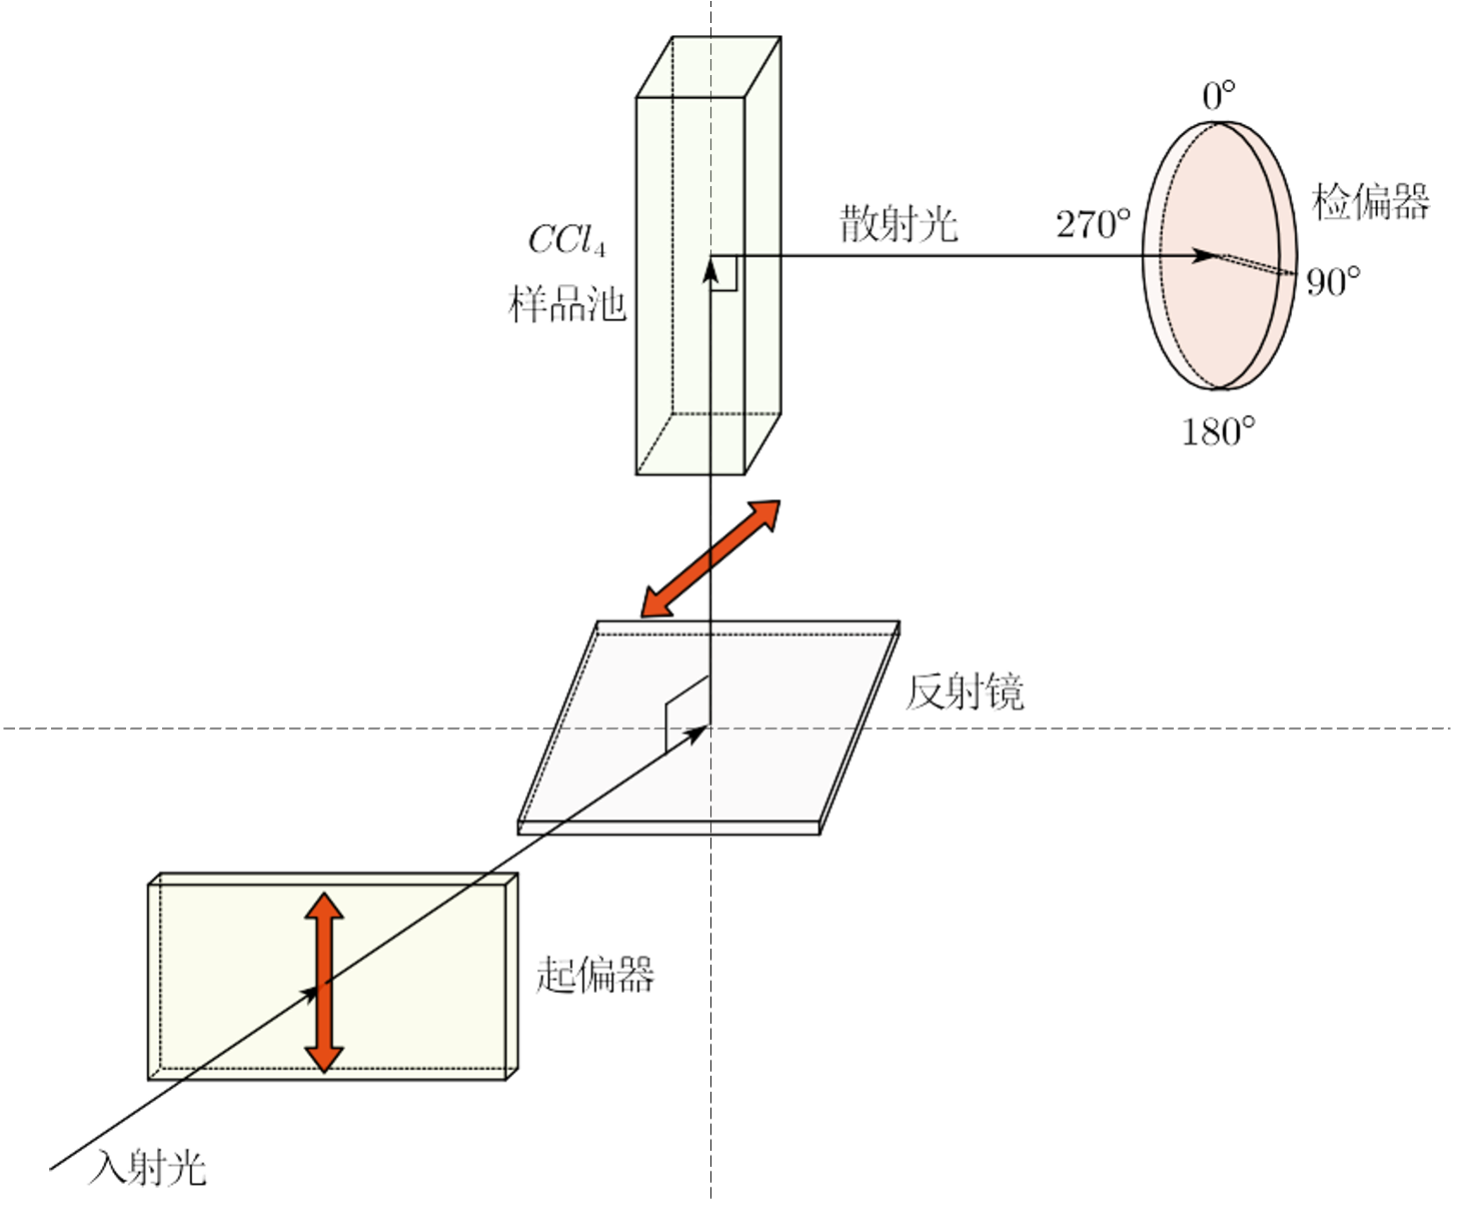
\includegraphics[width=0.6\textwidth]{图片 8.png} % Placeholder for Figure 8
    \caption{实验光路示意图}
    \label{fig:setup}
\end{figure}

\begin{figure}[h]
    \centering
    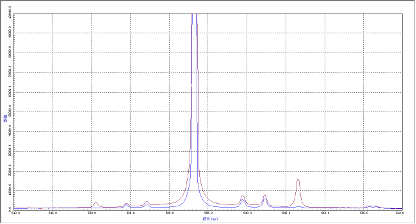
\includegraphics[width=0.8\textwidth]{图片 9.png} % Placeholder for Figure 9
    \caption{偏振片分别处于垂直角度时的光谱}
    \label{fig:polarization_spectra}
\end{figure}

\begin{figure}[h]
    \centering
    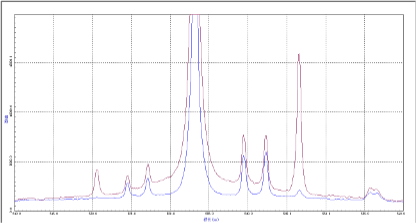
\includegraphics[width=0.8\textwidth]{图片 10.png} % Placeholder for Figure 10
    \caption{偏振片分别处于垂直角度时的光谱 (局部放大)}
    \label{fig:polarization_spectra_zoom}
\end{figure}

退偏度越小, 说明产生散射光的分子振动模式对称性越高。7 号峰 (546.5nm) 的退偏度最小, 为 0.13, 说明此波长的拉曼散射光对应的 CCl$_{4}$ 分子振动为演示程序中的“模式一”, 4 个 Cl 原子沿它们与中心 C 的连线振动。

\begin{table}[H]
    \centering
    \caption{峰位和峰高记录以及退偏度的计算}
    \begin{tabular}{cccccccccc}
        \toprule
        峰编号 & 1 & 2 & 3 & 4 & 5 & 6 & 7 & 8 & 9 \\
        \midrule
        峰位 (nm) & 520.5 & 524.6 & 527.2 & 533.3 & 539.4 & 542.3 & 546.7 & 555.8 & 556.6 \\
        0$^\circ$ 时峰高 & 1364.0 & 2848.6 & 3382.5 & 586581.1 & 5598.1 & 5943.5 & 2104.1 & 1911.5 & 1837.5 \\
        90$^\circ$ 时峰高 & 4228.0 & 3608.6 & 4811.7 & 1387046.8 & 7704.4 & 7646.0 & 15857.0 & 2322.4 & 2195.5 \\
        退偏度 & 0.32 & 0.79 & 0.70 & 0.42 & 0.73 & 0.78 & 0.13 & 0.82 & 0.84 \\
        \bottomrule
    \end{tabular}
    \label{tab:peak_values2}
\end{table}


\subsection{单光子计数器的进一步研究}

令单色仪光栅位于 555.8nm 附近, 再次利用阈值窗口测量此时的脉冲计数与脉冲幅度的分布曲线, 所得图像如 11 所示。对比之前无光条件下的结果, 可以发现曲线的形态出现了较大的差异, 峰宽变宽, 此时的阈值也增大到了 69。

\begin{figure}[H]
    \centering
     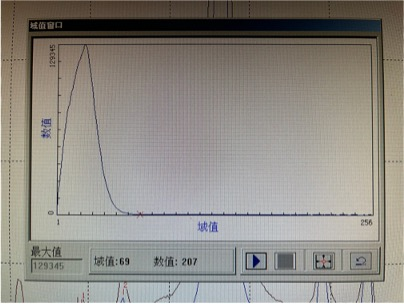
\includegraphics[width=0.8\textwidth]{图片 11.jpg} % Placeholder for Figure 11
    \caption{有光条件下的脉冲计数与脉冲幅度的分布曲线}
    \label{fig:pmt_light_count}
\end{figure}

\section{总结与建议}

\subsection{总结}

本次实验中, 我们用半导体激光器泵浦的 Nd$^{3+}$:YVO$_{4}$ 晶体并倍频后得到的 532nm 激光作为激发光源, 研究了液体样品 CCl$_{4}$ 分子的拉曼光谱。实验中观察到了瑞利散射峰和拉曼光谱, 不断优化光路以得到理想的结果。之后加上了偏振片, 研究了散射光的偏振特性, 并计算了每个峰的退偏度。最后在有光条件下再次打开阈值窗口, 对单光子计数器进行了进一步的研究。


\begin{thebibliography}{9}
\bibitem{ref:physics_lab} 北京师范大学物理实验教学中心. 近代物理实验讲义 [Z]. 北京: 北京师范大学物理学系, 2016.
\end{thebibliography}

\newpage
\section*{附录}
\begin{figure}[H]
    \centering
    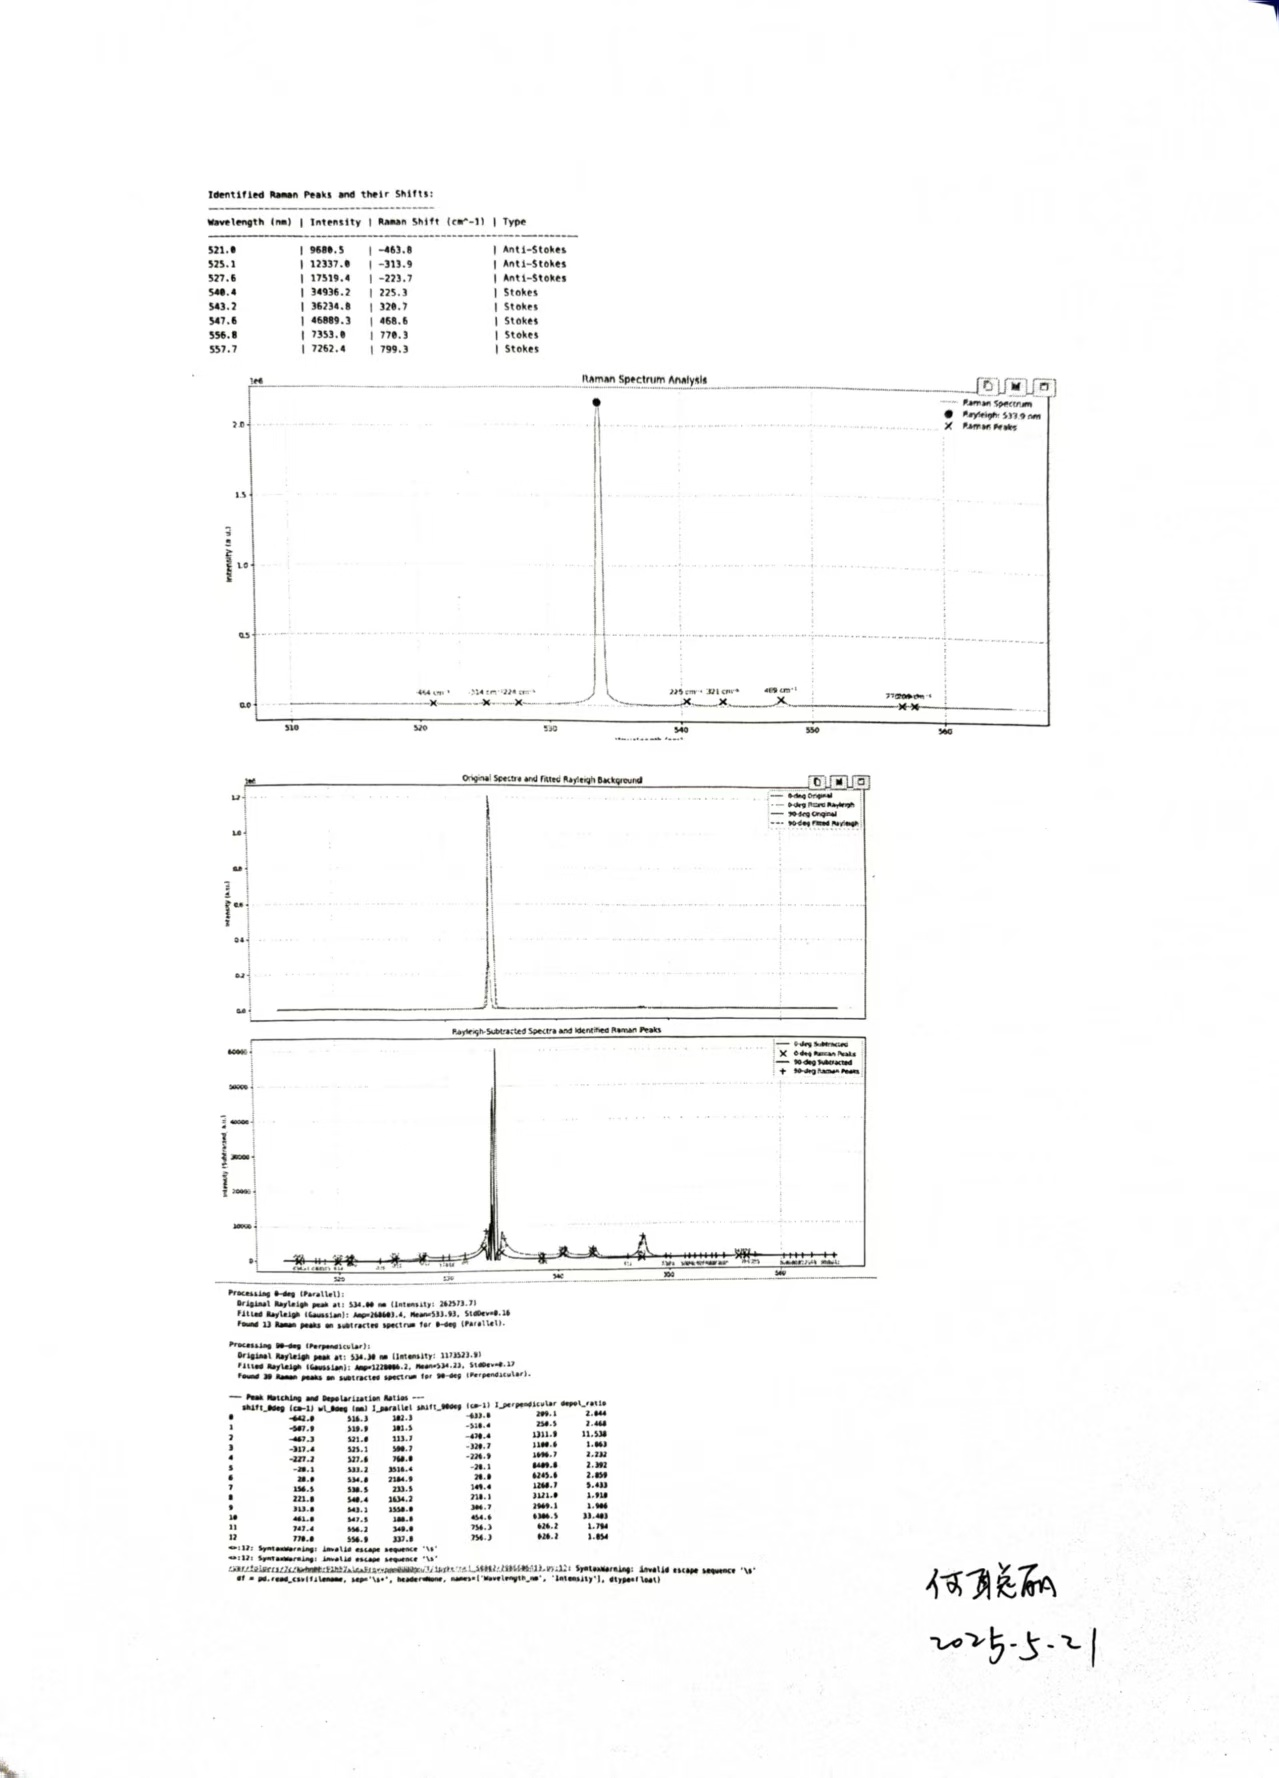
\includegraphics[width=0.9\textwidth]{data.jpg} % Placeholder for Appendix Figure
    \caption{原始数据}
    \label{fig:appendix_setup}
\end{figure}
\end{document}
